\documentclass[10pt]{beamer}

\usetheme[progressbar=frametitle]{metropolis}
\usepackage{appendixnumberbeamer}

\usepackage{booktabs}
\usepackage[scale=2]{ccicons}

\usepackage{pgfplots}
\usepgfplotslibrary{dateplot}

\usepackage{xspace}
\newcommand{\themename}{\textbf{\textsc{metropolis}}\xspace}

\title{JEE Linear Algebra using Matrix Computation}
\author{Harsh Raj  MA17BTECH11003 \\ \\ Lakshit Singla EE17BTECH11021}
\date{}
\begin{document}

\begin{frame}{}
\maketitle
\end{frame}


\begin{frame}[fragile]{Problem}
To find the equation of the circle, which is the mirror image of the circle
\[
\textbf{x}^{T}\textbf{x}  - \left( {\begin{array}{cc}
   2 & 0 \\
  \end{array} } \right)\textbf{x}=0
  \]
  in the line
  \[
   \left( {\begin{array}{cc}
   1 & 1 \\
  \end{array} } \right)\textbf{x}=3
  \]

\end{frame}


\begin{frame}[fragile]{Solution}
  General equation of circle with centre \( \textbf{C}_1\) and radius r :
\[\|\textbf{x}-\textbf{C}_1\|^2 = r^2
\] 
\[\Rightarrow
     (\textbf{x}-\textbf{C}_1)^{T}(\textbf{x}-\textbf{C}_1) = r^2
 \]
 \[ \Rightarrow
  \textbf{x}^{T}\textbf{x}-2\textbf{C}_1^{T}\textbf{x}=r^2-\textbf{C}_1^{T}\textbf{C}_1
\]
Comparing this equation with
\[ \textbf{x}^{T}\textbf{x}  - \left( {\begin{array}{cc}
   2 & 0 \\
  \end{array} } \right)\textbf{x}=0
\]
We have
\[ -2\textbf{C}_1^{T} = -  \left( {\begin{array}{cc}
   2 & 0 \\
  \end{array} } \right)
\]
and
\[
r^2 - \textbf{C}_1^{T}\textbf{C}_1 = 0
\]
\end{frame}


\begin{frame}{Contd.}
\[\Rightarrow
\textbf{C}_1^{T} =  \left( {\begin{array}{cc}
   1 & 0 \\
  \end{array} } \right)
\]
\[\Rightarrow
\textbf{C}_1 =  \left( {\begin{array}{c}
   1 \\
   0 \\
   \end{array} } \right)
\]
and
\[
r^2 = \textbf{C}_1^{T}\textbf{C}_1
\]
\[\Rightarrow
r^2 = \left( {\begin{array}{cc}
   1 & 0 \\
  \end{array} } \right)\left( {\begin{array}{c}
   1 \\
   0 \\
   \end{array} } \right)
\]
\[\Rightarrow
r^2 = 1
\]
\[\Rightarrow
r = 1
\]

\end{frame}


\begin{frame}{Contd.}
	Line in which image to be found:
	\[\textbf{L}:  \textbf{u}^{T}\textbf{x} = 3
	\]
	where \( \textbf{u} = \left( {\begin{array}{c}
   1 \\
   1 \\
   \end{array} } \right)\) \newline 
   \newline
   \newline
Let \( \textbf{C}_2 \) be the centre of the image circle.\newline
\(\textbf{E}\) and \( \textbf{F}\) be points on the Line \textbf{L}
\[\Rightarrow \textbf{u}^{T}\textbf{E} = 3 \enspace ;\enspace \textbf{u}^{T}\textbf{F} = 3 \]


\end{frame}




\begin{frame}{Contd.}
\[\Rightarrow \textbf{u}^{T}(\textbf{E}-\textbf{F}) = 0
\]
Since 
\[ \textbf{C}_2-\textbf{C}_1  \perp \textbf{E}-\textbf{F}
\]
\[\Rightarrow
(\textbf{C}_2-\textbf{C}_1)^{T}( \textbf{E}-\textbf{F})=0
\]
We know
\[\textbf{a}^{T}\textbf{b} = \textbf{c}^{T}\textbf{b} = 0  \Rightarrow \textbf{c} = \alpha\textbf{a} 
\]
Hence
\[\textbf{C}_2-\textbf{C}_1 = \alpha \textbf{u} 
\]
\[\Rightarrow \textbf{C}_2=\textbf{C}_1 + \alpha \textbf{u} 
\]
	
\end{frame}



\begin{frame}{Contd.}
Let \textbf{A} be the intersection point of line \textbf{L} and \(\textbf{C}_2-\textbf{C}_1 \)
\[\Rightarrow \textbf{A} =\textbf{C}_1 + \frac{\alpha\textbf{u}}{2}
\]
Point \(\textbf{A}\) lies on line \(\textbf{L}\)
\[\Rightarrow \textbf{u}^{T}\textbf{A} = 3
\]
\[\Rightarrow \textbf{u}^{T}(\textbf{C}_1 +\frac{\alpha\textbf{u}}{2} ) = 3
\]
\[\Rightarrow \textbf{u}^{T}\textbf{C}_1 + \frac{\alpha\textbf{u}^{T}\textbf{u}}{2} = 3
\]
\[\Rightarrow \left( {\begin{array}{cc}
   1 & 1 \\
  \end{array} } \right)\left( {\begin{array}{c}
   1  \\
   0 \\
  \end{array} } \right) + \frac{\alpha \left( {\begin{array}{cc}
   1 & 1 \\
  \end{array} } \right)\left( {\begin{array}{c}
   1  \\
   1 \\
  \end{array} } \right)}{2} = 3 
\]
\end{frame}




\begin{frame}[fragile]{Contd.}
\[\Rightarrow \alpha = 2
\]
We know
\[ \textbf{C}_2=\textbf{C}_1 + \alpha \textbf{u} 
\]
\[\Rightarrow \textbf{C}_2 = \textbf{C}_1 + 2\textbf{u}
\]
\[\Rightarrow \textbf{C}_2 =\left( {\begin{array}{c}
   1  \\
   0 \\
  \end{array} } \right)  + 2\left( {\begin{array}{c}
   1  \\
   1 \\
  \end{array} } \right)
\]
\[\Rightarrow \textbf{C}_2 =  \left( {\begin{array}{c}
   3  \\
   2 \\
  \end{array} } \right) 
\]
Clearly the radius of the image circle will as same of original circle


\end{frame}

\begin{frame}{Contd.}
Hence equation of Image circle:
\[ \|\textbf{x}-\textbf{C}_2\|^2 = r^2
\]
\[ \Rightarrow
  \textbf{x}^{T}\textbf{x}-2\textbf{C}_2^{T}\textbf{x}=r^2-\textbf{C}_2^{T}\textbf{C}_1
\]
\[\Rightarrow 
\textbf{x}^{T}\textbf{x} - \left( {\begin{array}{cc}
   6 & 4 \\
  \end{array} } \right)\textbf{x} + 12 = 0 
\]
 
\end{frame}

\begin{frame}{Graphical Verification in Python}
\begin{figure}[t]
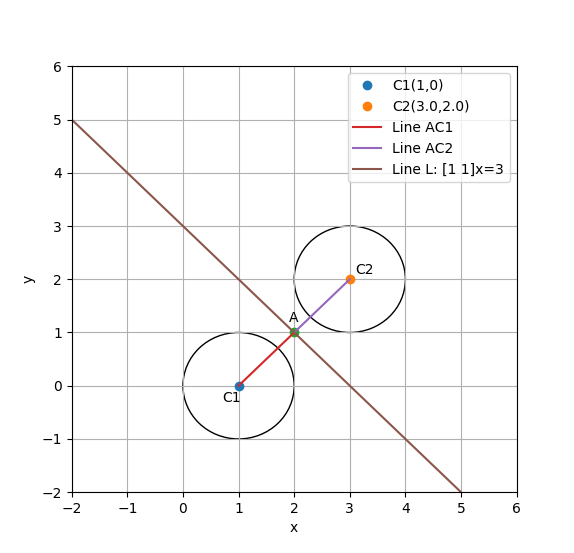
\includegraphics[scale = 0.40]{figure.png}
\caption{We can see that circles are mirror images in line L}
\end{figure}
\end{frame}

\end{document}
